量子线路是量子计算或量子算法中施加在量子比特上的量子门序列的图形化表示。类似于由逻辑门组成并操控经典比特的经典数字电路，量子线路由操控量子比特的量子门组成。

\subsubsection{构造量子线路}
在 \MindQuantum\ 中，我们使用 \Circuit\ 表示量子线路：

\begin{lstlisting}
from mindquantum.core.circuit import Circuit
circ = Circuit()
\end{lstlisting}

向 \Circuit\ 中添加量子门有几种基本操作：
\begin{itemize}
    \item list：使用量子门列表直接构造量子线路。
    \item \code{+=}：使用 \code{+=} 将量子门添加到线路中。
    \item \code{Circuit.x}：向线路中添加 X 门。
\end{itemize}
\begin{lstlisting}
from mindquantum.core.gates import H, Y, X, Z
circ = Circuit([X.on(0), Y.on(1)])
circ += H.on(0)
circ += Y.on(1, 0)
circ.x(1, 0)
circ.z(2, [0, 1])
\end{lstlisting}

结果如图~\ref{fig:Quantum-Circuit} 所示。

\subsubsection{展示量子线路}
SVG（Scalable Vector Graphics，可缩放矢量图形）基于 XML 标记语言，用于描述二维矢量图形。\MindQuantum\ 提供了将量子线路导出为 SVG 格式的函数。
\begin{lstlisting}
circ.svg().to_file(filename='circuit.svg')
\end{lstlisting}
\begin{figure}[h]
    \begin{center}
        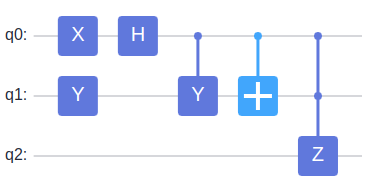
\includegraphics[width=0.9\linewidth]{images/2_4_circuit.png}
    \end{center}
    \caption{量子线路。}
    \label{fig:Quantum-Circuit}
\end{figure}
请注意，如果处于 Jupyter Notebook 环境中，可以直接通过 \code{circ.svg()} 获取 SVG 图像。


\subsubsection{常用接口}

量子线路是量子算法的基本元素，\MindQuantum\ 为 \Circuit\ 提供了许多实用方法。

\begin{itemize}
    \item \propnqubits：获取量子线路的量子比特数量。
    \item \propparamsname：获取线路中的参数名称。
    \item \prophasmeasuregate：获取线路是否包含测量门。
    \item \methodmatrix：获取线路矩阵。
    \item \methodgetqs：获取最终量子态。
    \item \methodsummary：获取当前线路的信息，包括模块数量、量子门数量、非参数化量子门数量、参数化量子门数量以及参数数量。
\end{itemize}

\subsubsection{量子线路上的高级操作}

构造大规模量子线路并不总是直接明了。为此，\MindQuantum\ 提供了一些预定义方法，使 \Circuit\ 更加易用。例如，设原始量子线路为：

\begin{lstlisting}
from mindquantum.core.circuit import *

circ = Circuit().h(0).rx('a', 2, 0)
\end{lstlisting}

\begin{figure}[H]
    \begin{center}
        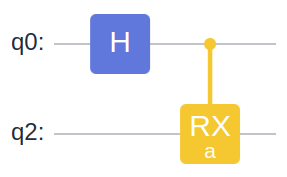
\includegraphics[width=0.4\linewidth]{images/2_4_ori_circ.png}
    \end{center}
    \caption{待操作的量子线路。}
\end{figure}
下面展示如何对该量子线路进行操作：


\begin{enumerate}
    \item \methodcompress{circ}：将所有量子比特压缩到前 $n$ 个量子比特上。\par
          \begin{minipage}{\linewidth}
              \centering
              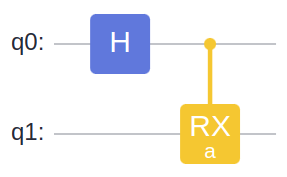
\includegraphics[width=0.4\linewidth]{images/2_4_compress_circ.png}
          \end{minipage}
    \item \methodcontrol{circ}{1}：为该线路添加控制量子比特。\par
          \begin{minipage}{\linewidth}
              \centering
              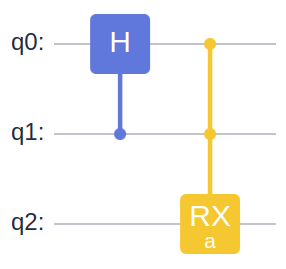
\includegraphics[width=0.4\linewidth]{images/2_4_ctrl_circ.png}
          \end{minipage}
    \item \methoddagger{circ}：获取厄米共轭版本。\par
          \begin{minipage}{\linewidth}
              \centering
              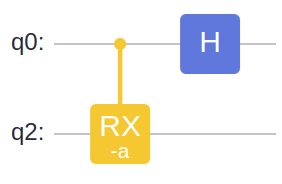
\includegraphics[width=0.4\linewidth]{images/2_4_dagger_circ.png}
          \end{minipage}
    \item \methodapply{circ}{[2, 1]}：将线路应用到其他量子比特上。\par
          \begin{minipage}{\linewidth}
              \centering
              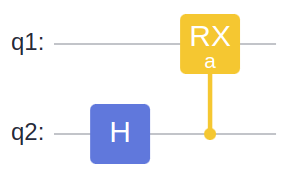
\includegraphics[width=0.4\linewidth]{images/2_4_apply_circ.png}
          \end{minipage}
    \item \methodreverse{circ}：反转线路中的量子比特顺序。\par
          \begin{minipage}{\linewidth}
              \centering
              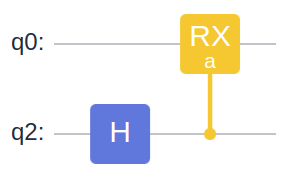
\includegraphics[width=0.4\linewidth]{images/2_4_reverse_circ.png}
          \end{minipage}
    \item \methodshift{circ}{2}：按给定步长平移量子比特范围。\par
          \begin{minipage}{\linewidth}
              \centering
              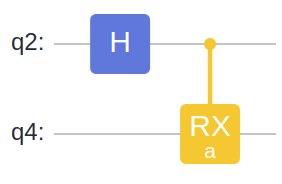
\includegraphics[width=0.4\linewidth]{images/2_4_shift_circ.png}
          \end{minipage}
\end{enumerate}
